%!TEX root = ../thesis.tex

% ------------------ Literature ------------------ %
Langran 1989
Peuquet 1994
Wachowitz 1999
Yuan 1999
Peuquet 2002

% http://link.springer.com/article/10.1007/s12145-009-0027-6/fulltext.html
% http://stackoverflow.com/questions/5863676/table-design-for-spatio-temporal-data

Multidimensional Geographic Information Science (Raper, 2001)
\cite{raper2000multidimensional}

whole book:
\cite{Langran1989timeingis}

chapters:
1 Fuzzs Sets ...
Spatio-Temporal Databases (Caluwe et al, 2010)
-> ontology of imperfection
\cite{deCaluwe:2010:SDF:1965517}


% ------------------------------------------------------------------------------
HGIS react on the spatial turn of history: the integration of geographic methods in historical research. It aims to discover the power of cartographic representation: ``The spatial turn in the humanities must [...] understand the role of space in human events''
\cite{bodenhamer2010spatial}.
At the same time, they are the product of the temporal run in GIS: the coexistence of space (where things are) and time (what has changed over time)
\cite[p. 45]{solana2014spatio}.

Since ``the world never stands still'', but ``the retention of information relating to past events [is] an important element of human representation of the world'', the dimension of time has to be integrated into a GIS
\cite{peuquet99}.

HGIS are rather recent tools and used mostly in \emph{Digital Humanities} as a digital tool to answer research questions in the traditional fields of humanities: ``situating history in its geographical context and using geographic information to illuminate the past''
\cite[p. 3]{knowles2008placing}.
Some interesting research questions that could be answered using HGIS could be:

\begin{compactitem}
  \item Did the European Union help to bring peace on the European continent?
  \hfill \emph{(political)}
  \item Is there a coherence between life expectancy and fertility rate?
  \hfill \emph{(social)}
  \item What is the effect of global warming on the melting of glaciers?
  \hfill \emph{(physical)}
  \item What was the effect of Bismarck's foreign policy on peace in Europe?
  \hfill \emph{(historical)}
\end{compactitem}

Or on a more abstract level: Where and When has something changed and why did it change?

\begin{enumerate}
  \item \textbf{Input}: Primary acquision of spatio-temporal data, i.e. historical events, historical and current countries and their territories.
  \item \textbf{Management}: Physical storage and logical management of the data in a spatio-temporal database, using a structure that fits the spatio-temporal data model.
  \item \textbf{Analysis}: Gaining spatio-temporal information by cleaning, transforming or combining the data in database.
  \item \textbf{Presentation}: Visualization of information on different displays, e.g. a map and a timeline, transforming information into spatio-temporal knowledge.
\end{enumerate}

% ------------------------------------------------------------------------------

A famous visualization combining time and space is ``Napoleons Moscow Campaign'' by Charles Minard from 1869 (see figure \ref{fig:minard_napoleon}). The ``best statistical graphic ever drawn''
\footnote{
  \emph{The Visual Display of Quantitative Information} (p. 40),
  Edward R. Tufte,
  2001
}
shows the size of the army in Napoleon’s 1812 Russian campaign, their movements and temperature on in one graph
\cite[pp. 188-191]{knowles2008placing}.

\begin{figure}[ht]
  \centering
  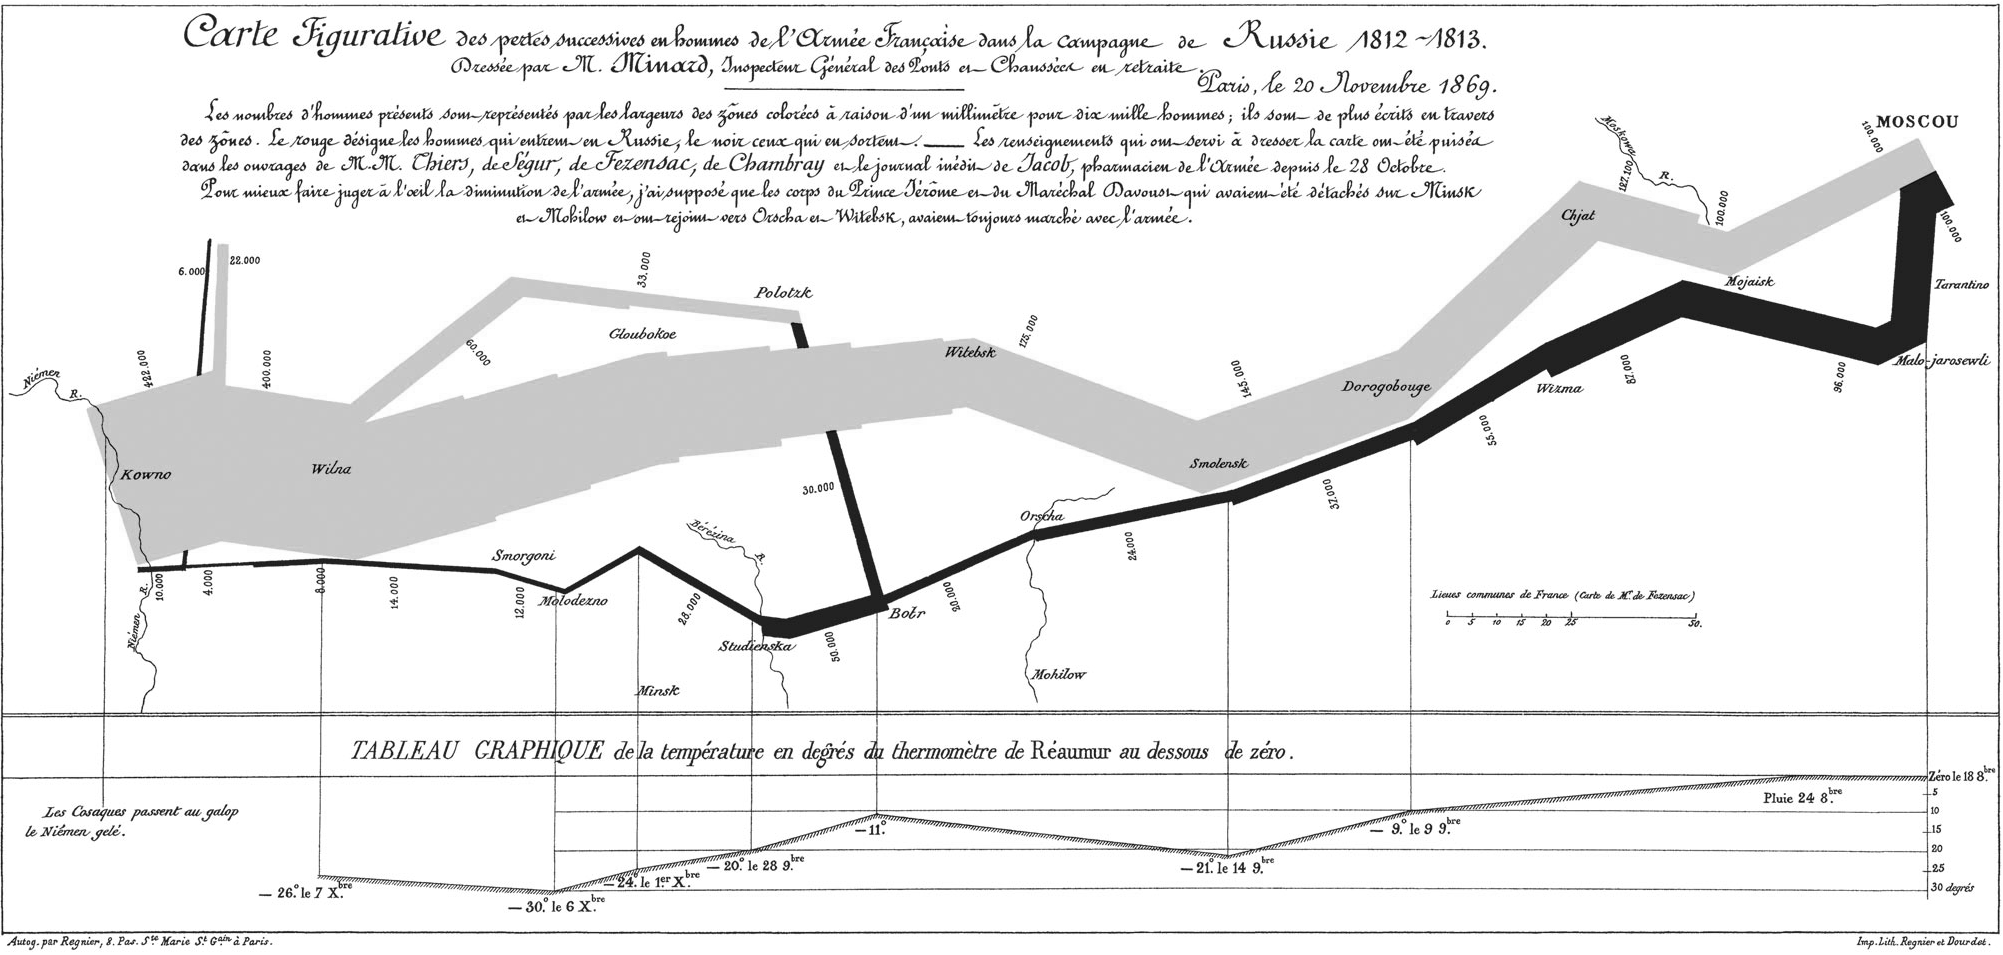
\includegraphics[width=0.8\textwidth]{graphics/basics/napoleon_march_moscow.png}
  \caption{Napoleons Moscow Campaign \protect\footnotemark}
  \label{fig:minard_napoleon}
\end{figure}

\footnotetext{
  \emph{Minard.png}
  Charles Minard, 1869,
  URL: \url{https://commons.wikimedia.org/wiki/File:Minard.png},
  last access: 03.11.2015,
}

% ==============================================================================


% temporal domain
%   linear time
%     time line
%     time series: graph (t,y coordinate system)
%     2.5D map: temporal dimension on z axis or on surface
%     space-time path
%   cyclic time
%     time series: polar diagram
%     time wheel
%   both
%     mono-temporal: one layer -> one time point
%     multi-temporal: one layer -> multiple time points
% \cite[p. 144]{ott2001time}

% paragraph timelines (end)


% - - - - - - - - - - - - - - - - - - - - - - - - - - - - - - - - - - - - - - -
% \paragraph{Geospatial Topology} % (fold)
% \label{par:geospatial_topology}

% \emph{Topology} is the study of position, how objects are spatially arranged and relatively positioned to each other. It does not include measures like distances or angles. Two objects are said to be topologically equivalent, if they can be deformed into each other, e.g. an ellipse can be stretched into a circle. A \emph{geospatial topological vector model} defines the relationship between geospatial objects, i.e. equals, disjoint, intersects, touches / neighbors, contains, covers, within, interior and boundary
% \cite{clementiniTopology}.

% The 2D vector model can be extended with a topology. The elements in this topological space are nodes (0D), edges (1D) and meshes (2D) and they correspond directly to the geometric primitives stated above. A topological vector model has strict connectivity (a ``clean'' geometry), if no two edges intersect without a node at their intersection point (planar), each interior edge has exactly two adjacent areas and each edge contains at least two nodes
% \cite[pp.37-39]{bolstad2008gis}.

% \begin{figure}[ht]
%   \centering
%   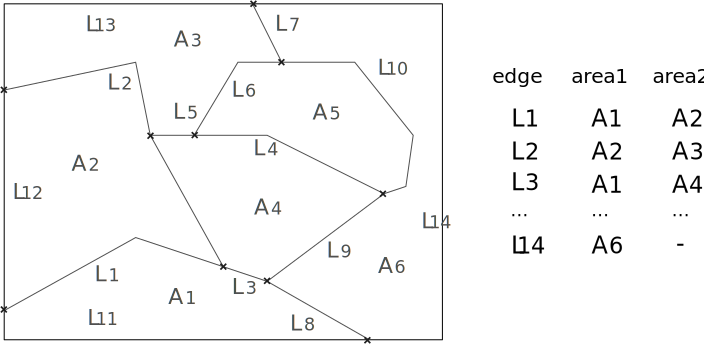
\includegraphics[width=0.55\textwidth]{graphics/basics/topological_vector_model}
%   \caption{An example of a topological vector model and an adjacancy table}
%   \label{fig:topological_vector_model}
% \end{figure}

% The topological vector model has a great asset: if an edge between two adjacent areas changes, the connectivity and adjacency does not change and therefore also the topology stays constant. The lookup for neighboring areas is very fast if the topology ensures strict connectivity: The neighbors of an area can be found in the adjacency table. Potentially problematic is the creation of a clean geometry: it can be cumbersome and require a lot of manual adjustment, for example ensuring strict connectivity by manually connecting nodes.

% % paragraph geospatial_topology (end)

% % subsection model_of_geographical_space (end)


% \begin{figure}[H]
%   \centering
%   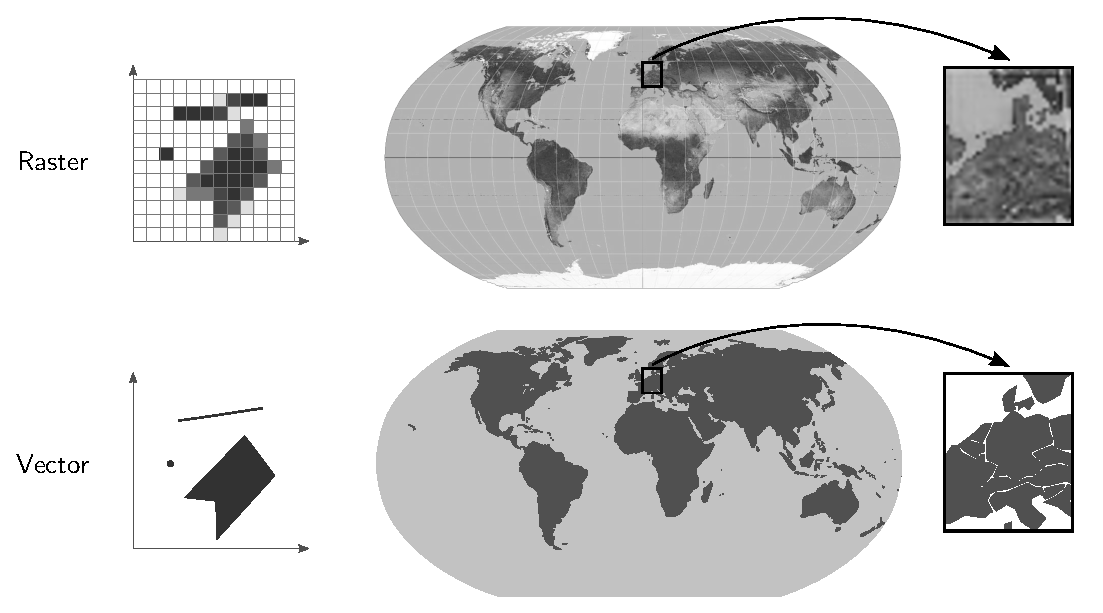
\includegraphics[width=0.75\textwidth]{graphics/basics/hgis/raster_vector}
%   \caption{Comparison of the raster and the vector model}
%   \label{fig:raster_vector}
% \end{figure}

% The \emph{raster model} contains a regular grid with a fixed \emph{cell dimension}. Each cell has a certain value, e.g. a color value.
% The model is simple and allows straightforward rendering: only affine transformations have to be applied in order to project two raster map layers on top of each other. The main disadvantage of the raster model is its fixed resolution: it can not be scaled up without losing quality
% \cite[pp.42-48]{bolstad2008gis}.
% Raster graphics are used for map tiles by most map engines, e.g. the satellite image by NASA in Google Maps.
% \footnote{
%   \emph{Google Maps},
%   URL: \url{https://www.google.com/maps/@51.2090662,13.2328189,3563505m/data=!3m1!1e3},
%   Imagery \textcopyright2015 Landsat, Data SIO, NOAA, U.S. Navy, NGA, GEBCO, IBCAO, U.S. Geological Survey, Map data \textcopyright2015 Google, ORION-ME,
%   last access: 29.10.2015
% }.


For time spans, there are six possibile temporal topological relations (table \ref{tab:temporal_relations}). Except for \texttt{equals}, each of them has an inverse, yielding a total of 13 different relations.

\begin{table}[H]
\begin{center}
\begin{tabular}{c c c}
    % \toprule
    relation & symbol & visualization \\
    \midrule
    $X$ before $Y$ &    \texttt{X < Y} & \raisebox{-0.25\height}
    {
\includegraphics{graphics/basics/temporal_relations/before}} \\
    $X$ meets $Y$ &     \texttt{X m Y} & \raisebox{-0.25\height}
    {
\includegraphics{graphics/basics/temporal_relations/meets}} \\
    $X$ overlaps $Y$ &  \texttt{X o Y} & \raisebox{-0.25\height}
    {
\includegraphics{graphics/basics/temporal_relations/overlaps}} \\
    $X$ equals $Y$ &    \texttt{X = Y} & \raisebox{-0.25\height}
    {
\includegraphics{graphics/basics/temporal_relations/equals}} \\
    $X$ starts $Y$ &    \texttt{X s Y} & \raisebox{-0.25\height}
    {
\includegraphics{graphics/basics/temporal_relations/starts}} \\
    $X$ during $Y$ &    \texttt{X d Y} & \raisebox{-0.25\height}
    {
\includegraphics{graphics/basics/temporal_relations/during}} \\
    $X$ ends $Y$ &      \texttt{X e Y} & \raisebox{-0.25\height}
    {
\includegraphics{graphics/basics/temporal_relations/ends}} \\
    % \bottomrule
\end{tabular}
\caption{Temporal relations of time spans, based on \cite{allen84}}
\label{tab:temporal_relations}
\end{center}
\end{table}

% paragraph temporal_relations (end)